\begin{frame}
    \frametitle{Once-through feed uranium}
    \begin{figure}
        \centering 
        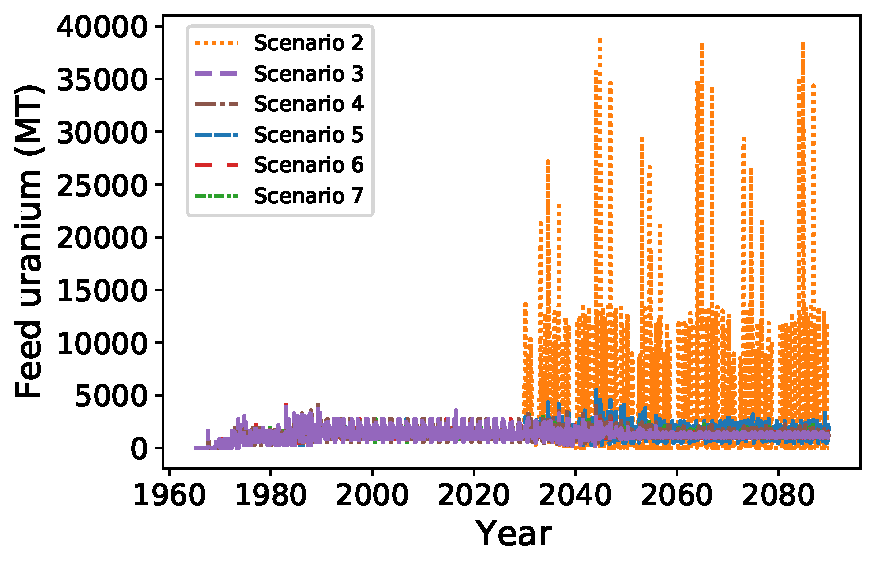
\includegraphics[scale=0.5]{nogrowth_feed.pdf}
    \end{figure}
\end{frame}

\begin{frame}
    \frametitle{Recycle HLW}
    \begin{figure}
        \centering
        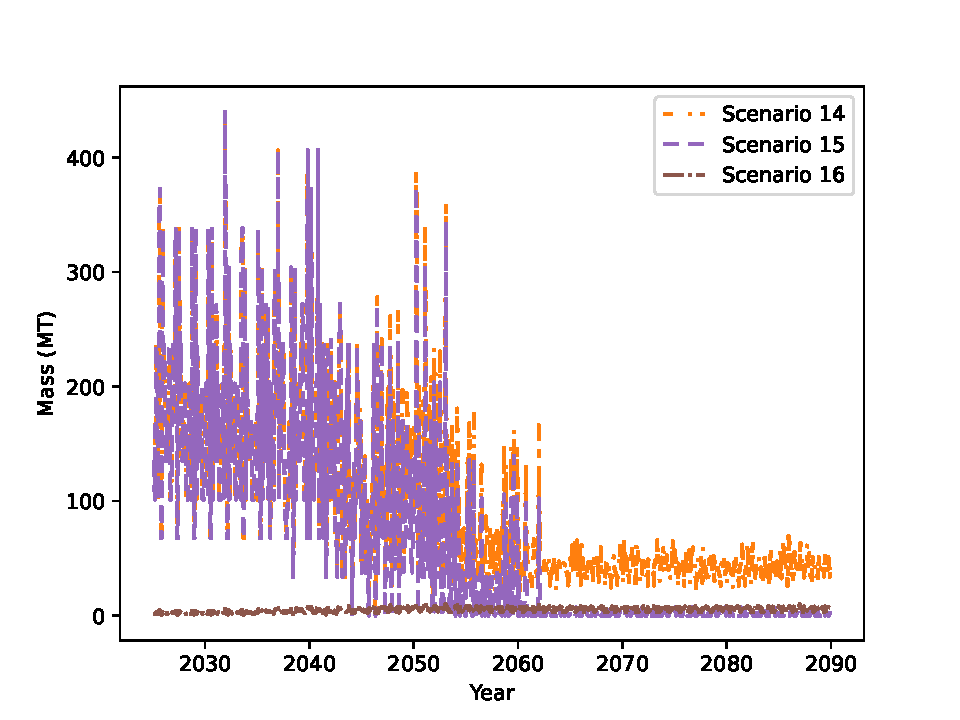
\includegraphics[scale=0.5]{nogrowth_recycle_hlw.pdf}
    \end{figure}
\end{frame}

\begin{frame}
    \frametitle{Recycle SNF}
    \begin{figure}
        \centering
        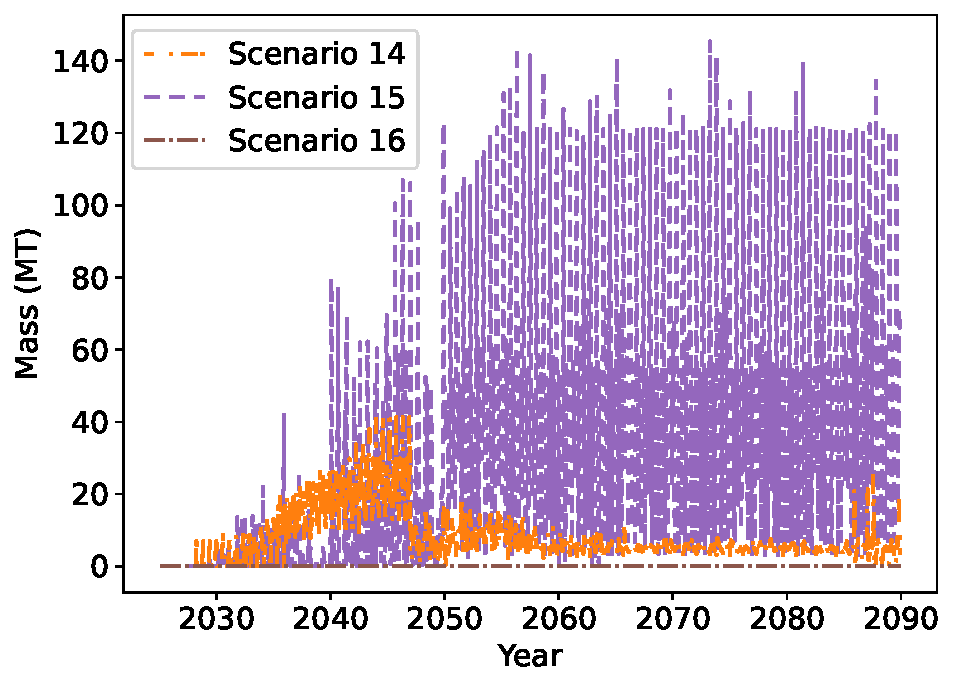
\includegraphics[scale=0.5]{nogrowth_recycle_snf.pdf}
    \end{figure}
\end{frame}

\begin{frame}
    \frametitle{Recycle SWU}
    \begin{figure}
        \centering
        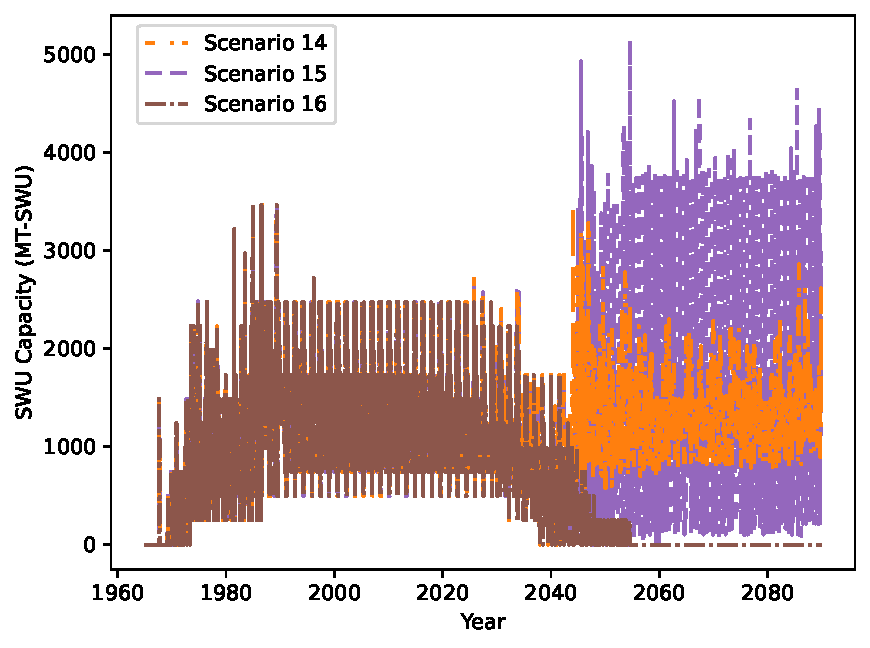
\includegraphics[scale=0.5]{nogrowth_recycle_swu.pdf}
    \end{figure}
\end{frame}

\begin{frame}
    \frametitle{Effects of varying VOYGR build share}
    \begin{figure}
        \centering
        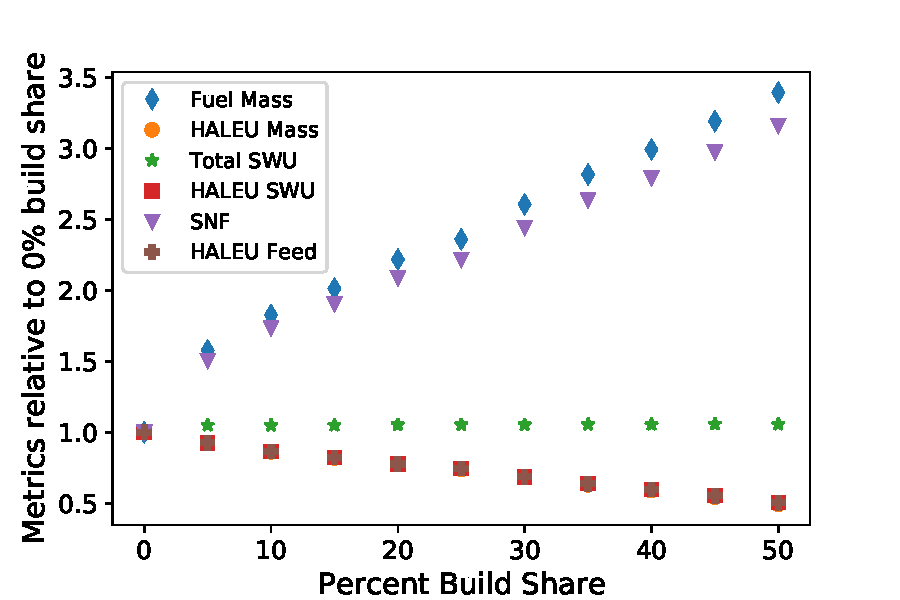
\includegraphics[scale=0.5]{voygr.pdf}
    \end{figure}
\end{frame}

\begin{frame}
    \frametitle{Effects of varying MMR build share}
    \begin{figure}
        \centering
        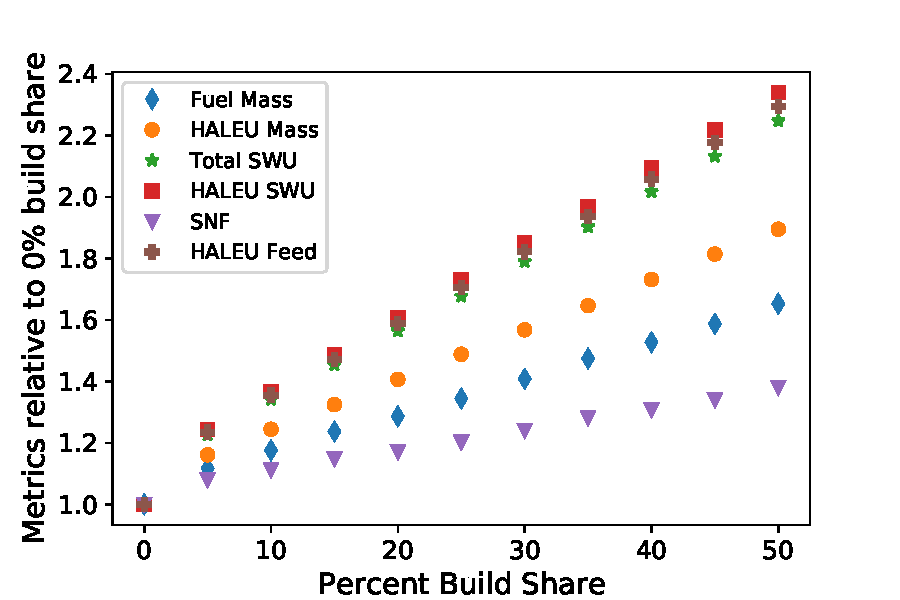
\includegraphics[scale=0.5]{mmr.pdf}
    \end{figure}
\end{frame}

\begin{frame}
    \frametitle{Xe-100 \keff and \betaEff}
    \begin{columns}
        \column[t]{5cm}
        \begin{table}[ht]
            \centering 
            \caption{\keff values for the Xe-100-like reactor model for 
            each fuel composition.}
            \label{tab:xe100_keff}
            \vspace{-0.37cm}
            \begin{tabular}{c c}
                    \hline
                    Fuel composition & \keff \\
                    \hline 
                    Pure & 1.06663 $\pm$ 0.00016\\
                    \gls{EBR} & 1.08086 $\pm$ 0.00016\\
                    Y-12 & 1.08016 $\pm$ 0.00014\\
                    \hline                
            \end{tabular}
        \end{table}

        \column[t]{5cm}
        \begin{table}[ht]
            \centering 
            \caption{\betaEff value from using each fuel type.}
            \label{tab:betaeff_xe100}
            \begin{tabular}{c c}
                    \hline
                    Fuel type & \betaEff \\
                    \hline
                    Pure & 0.00617 $\pm$ 0.00003 \\
                    \gls{EBR} & 0.00604 $\pm$ 0.00003 \\
                    Y-12 & 0.00598 $\pm$ 0.0002 \\
                    \hline
            \end{tabular}
        \end{table}
    \end{columns}
\end{frame}

\begin{frame}
    \frametitle{Axial flux through Xe-100}
    \begin{figure}
        \centering 
        \begin{subfigure}{0.49\textwidth}
            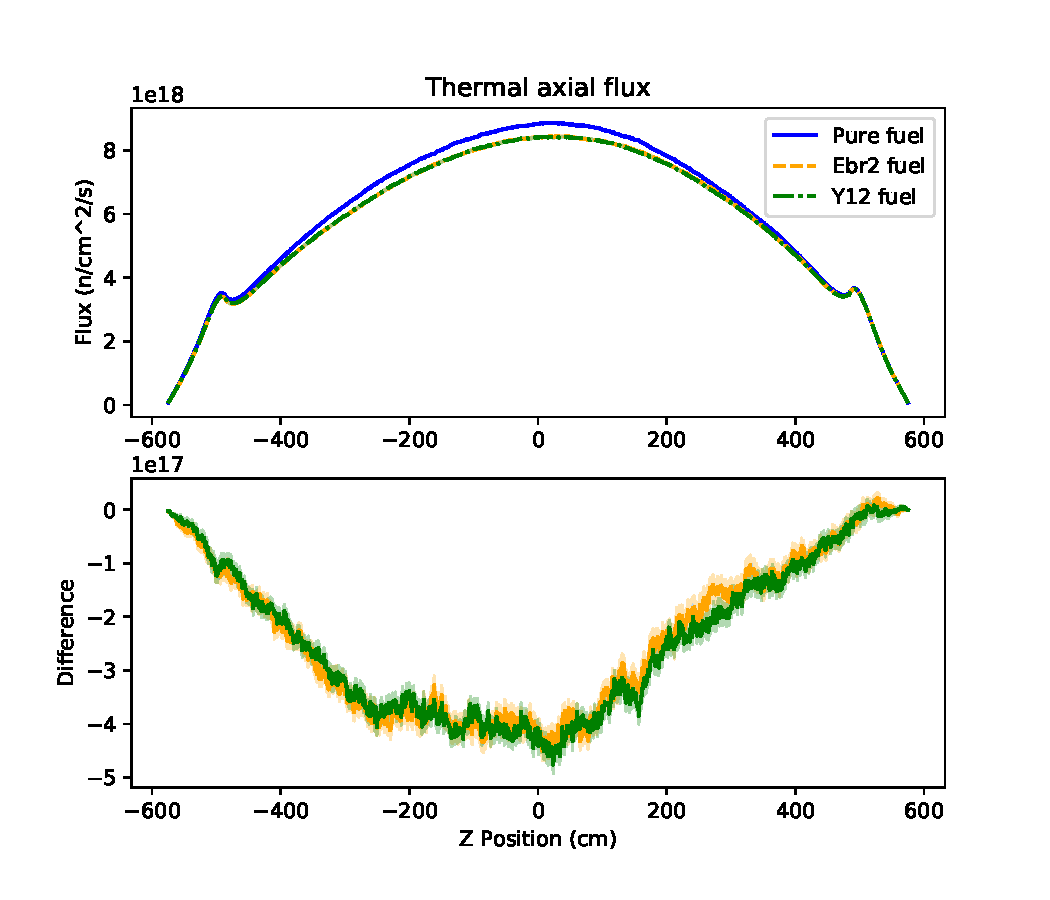
\includegraphics[scale=0.35, trim=20 10 10 20,clip]{xe100_thermal_axial.pdf}
        \end{subfigure}
        \begin{subfigure}{0.49\textwidth}
            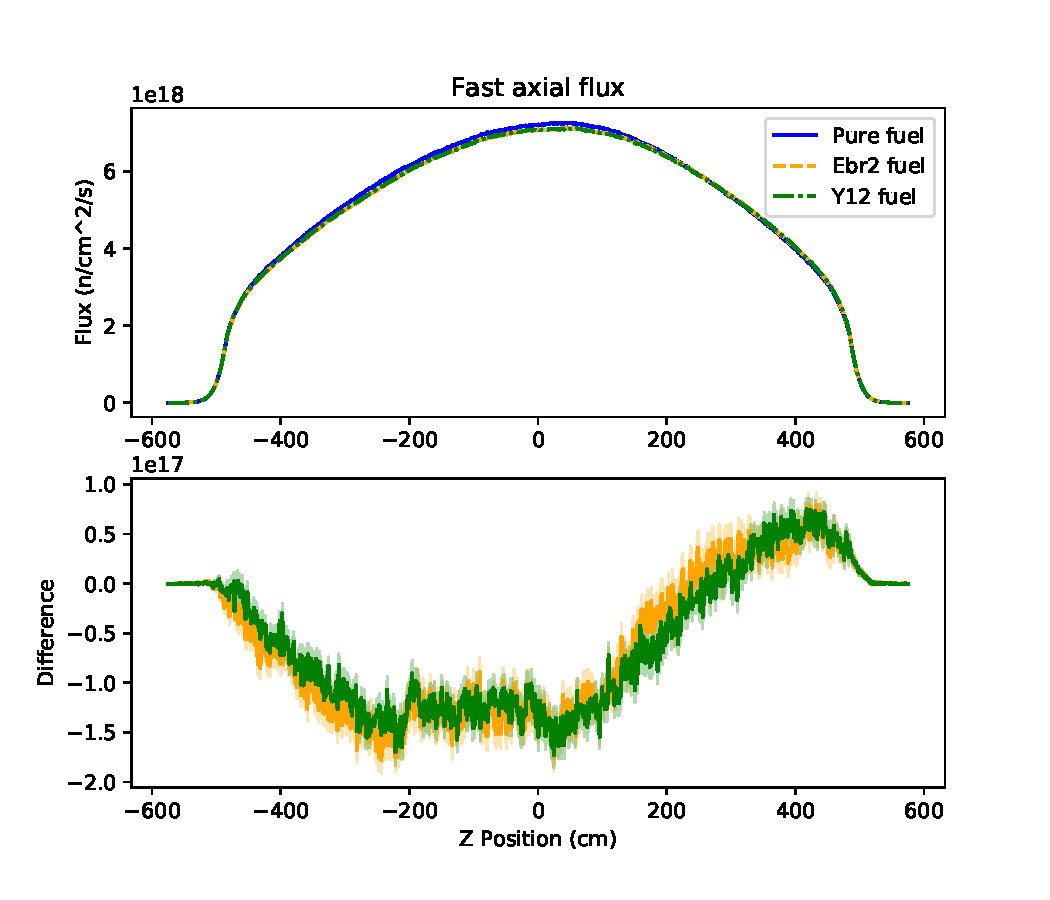
\includegraphics[scale=0.35, trim=10 10 10 20,clip]{xe100_fast_axial.pdf}
        \end{subfigure}
        \caption{Axial fluxes through Xe-100.}
        \label{fig:xe100-axial-flux}
    \end{figure}
\end{frame}

\begin{frame}
    \frametitle{Reactivity feedback coefficients for Xe-100}
    \begin{table}[ht]
        \centering
        \caption{Reactivity temperature feedback coefficients for 
        each material type in the Xe-100-like model for each fuel 
        type.}
        \label{tab:coeff_xe100}
        \begin{tabular}{c c c c c}
            \hline 
            & \multicolumn{4}{c}{Material feedback coefficient (pcm/K)} \\
            Fuel Type & Fuel & Coolant & Moderator & Total \\
            \hline
            Pure & -3.875 $\pm$ 0.094 & -0.044 $\pm$ 0.112 & -0.071 $\pm$ 0.459 & -4.216 $\pm$ 0.502\\
            \gls{EBR} & -3.759 $\pm$ 0.138 & -0.433 $\pm$ 0.048 & -0.708 $\pm$ 0.404 & -4.817 $\pm$ 0.438\\
            Y-12 & -3.797 $\pm$ 0.157 & -0.351 $\pm$ 0.092 & -0.728 $\pm$ 0.469 & -4.700 $\pm$ 0.349\\
            \hline

        \end{tabular}
\end{table}
\end{frame}